% -------------------------------------------------------
% Importations
% -------------------------------------------------------

\documentclass[a4paper,12pt]{article}

\usepackage{natbib}
\usepackage[utf8]{inputenc}
\usepackage[T1]{fontenc}
\usepackage[french]{babel}
\usepackage{geometry}
\usepackage{graphicx}
\usepackage{array}
\usepackage{booktabs}
\usepackage{tabularx}
\usepackage{times}       % Police Times New Roman
\usepackage{hyperref}
\usepackage{ragged2e}
\usepackage{amsmath}
\usepackage{amssymb}
\usepackage[automake, nonumberlist]{glossaries-extra}
\makeglossaries

% -------------------------------------------------------
% Définitions
% -------------------------------------------------------
\newglossaryentry{arn}{
    name = {ARN},
    description = {Acide ribonucléique, molécule fondamentale du vivant, composée de nucléotides}
}
\newglossaryentry{nucleotides}{
    name = {Nucléotides},
    description = {Partie constituante d'une molécule d'ARN, composée d'une base azotée, un cycle carbonné et d'une dorsale. Deux nucléotides forment un bi-nucléotide et trois un tri-nucléotide}
}
\newglossaryentry{pca-like}{
    name = {PCA-like},
    description = {Méthode de réduction de dimension faisant intervenir une méthode proche à celle d'un PCA}
}
\newglossaryentry{tlinéaire}{
    name = {T-linéaire},
    description = {Corrélation linéaire ajustée pour le tore}
}
\newglossaryentry{tconcordance}{
    name = {T-concordance},
    description = {Corrélation du sens de rotation des angles, T-concordant si le sens est le même et T-discordant s'il est inverse}
}
\newglossaryentry{fonction_dordre_circulaire}{
    name = {Fonction d’ordre circulaire},
    description = {Fonction déterminant le sens ou l'absence de rotation entre deux angles}
}
\newglossaryentry{conformation}{
    name = {Conformation},
    description = {Forme de la molécule dans l'espace issue des différents angles que prennent les liaisons dans la molécule}
}
\newacronym{geopca}{GeoPCA}{Geodesic Principal Component Analysis}
\newacronym{tpca}{T-PCA}{Torus Principal Component Analysis}
\newacronym{umap}{UMAP}{Uniform Manifold Approximation and Projection}
\newacronym{tsne}{t-SNE}{t-distributed Stochastic Neighbor Embedding}
\newacronym{hdbscan}{HDBSCAN}{Hierarchical Density-Based Spatial Clustering of Applications with Noise}



\geometry{
    a4paper,
    top=2.5cm, bottom=2.5cm,
    left=2.5cm, right=2.5cm
}
\pagestyle{empty}

\begin{document}



% -------------------------------------------------------
% Haut de page de garde
% -------------------------------------------------------

\noindent
\begin{minipage}[c]{0.28\textwidth}
    
\includegraphics[height=2cm]{ubs-faculte-ssi-logo-rvb.jpg}
\end{minipage}%
\hfill
\begin{minipage}[t]{0.38\textwidth}
    \centering
    {\fontsize{14}{17}\selectfont Année 2025/2026}\\[0.6cm]
    {\fontsize{14}{17}\selectfont \textbf{MASTER 2}}\\[0.4cm]
    {\fontsize{12}{15}\selectfont Mathématiques appliquées et statistiques}\\[0.3cm]
    Spécialité\\[0.2cm]
    {\large \textbf{Data Science et Modélisation Statistique}}\\[0.6cm]
    {\textbf{Rapport de mi-stage}}\\[0.3cm]
    {\fontsize{15}{17}\selectfont \textbf{Compte-rendu des travaux effectués pendant la première partie du stage}}
\end{minipage}%
\hfill
\begin{minipage}[c]{0.25\textwidth}
    \raggedleft
    
\includegraphics[height=2.4cm]{Ensai-logo.png}\\[4pt]
    
\includegraphics[height=1.3cm]{logo_LAAS.png}
\end{minipage}

\vspace{1.5cm}

% -------------------------------------------------------
% Tableau d'informations
% -------------------------------------------------------

\renewcommand{\arraystretch}{1.6}
\begin{tabularx}{\textwidth}{|>{\bfseries}p{4cm}|X|}
    \hline
    Étudiant
        & Wandrille BUCHY \\
        & \href{mailto:buchy.e2403788@etud.univ-ubs.fr}{buchy.e2403788@etud.univ-ubs.fr} \\
    \hline
    Laboratoire d'accueil
        & École Nationale de la Statistique et de l'Analyse de l'Information (ENSAI) \\
        & Département de Statistique \\
        & ENSAI -- 51 rue Blaise Pascal -- 35170 BRUZ \\
    \hline
    Maîtres de stage
        & Javier GONZÁLEZ-DELGADO, Enseignant-chercheur \\
        & \href{mailto:javier.gonzalez-delgado@ensai.fr}{javier.gonzalez-delgado@ensai.fr} \\[4pt]
        & Juan CORTÉS, Enseignant-chercheur \\
        & \href{mailto:juan.cortes@laas.fr}{juan.cortes@laas.fr} \\
    \hline
    Référent à l'université
        & Matthieu MARBAC, Enseignant-chercheur \\
        & \href{mailto:matthieu.marbac@univ-ubs.fr}{matthieu.marbac@univ-ubs.fr} \\
    \hline
    Date de la soutenance
        & À définir \\
    \hline
\end{tabularx}

\vfill

% -------------------------------------------------------
% Pied de page de garde
% -------------------------------------------------------

\noindent\rule{\textwidth}{0.4pt}
\begin{flushleft}
    \small
    Université de Bretagne-Sud -- UFR Sciences et Sciences de l'ingénieur\\
    Département Mathématique, Informatique, Statistique\\
    Rue Yves Mainguy -- 56000 Vannes -- France\\
    \href{http://www.univ-ubs.fr}{www.univ-ubs.fr}
\end{flushleft}

% -------------------------------------------------------
% Sommaire
% -------------------------------------------------------

\newpage
\tableofcontents


% -------------------------------------------------------
% Glossaire
% -------------------------------------------------------
\newpage
\printglossaries
\glsaddall

\vspace{8cm}
\noindent\rule{\textwidth}{0.4pt}
\vspace{0.3cm}

\noindent\textbf{Mots-clés :} ARN, tore, réduction de dimension, angles dihédraux, clustering, transport optimal

% -------------------------------------------------------
% Rédaction
% -------------------------------------------------------

\newpage

\pagestyle{plain}

\section{Introduction}

Les angles dihédraux de la molécule d'ARN sont au nombre de 12, répartis sur 
les 3 parties du nucléotide comme illustré sur la Figure~\ref{fig:1}. La première partie est la dorsale où l'on retrouve 
6 angles $\alpha$, $\beta$, $\gamma$, $\delta$, $\epsilon$ et $\zeta$, la 
deuxième est le cycle carbonné avec les 5 angles $\nu_1$ à $\nu_5$, enfin la base qui possède un angle de rotation $\chi$. 
L'étude de ces angles, tous définis dans $\mathbb{S}^1$, est donc une étude de 
$(\mathbb{S}^1)^{12} := \mathbb{T}^{12}$, le tore de dimension 12.

\begin{figure}[h]
    \centering
    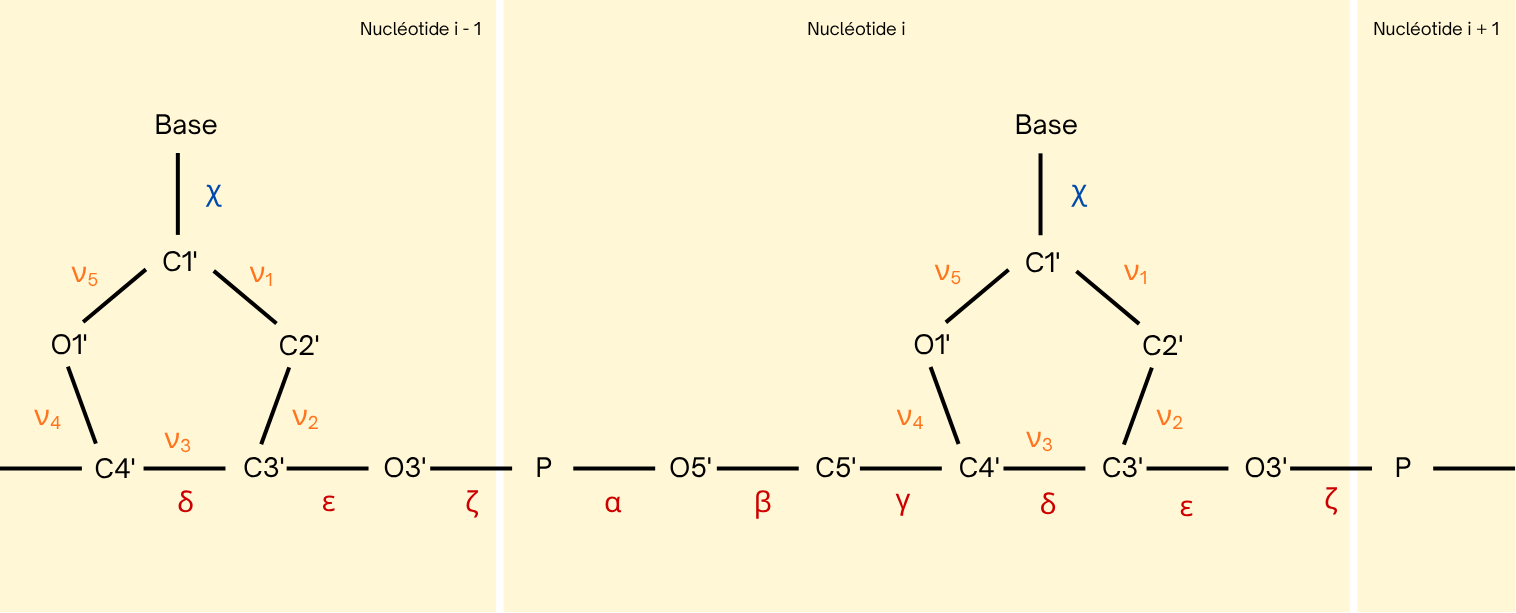
\includegraphics[width=0.7\textwidth]{Schéma molécule ARN.png}
    \caption{Schéma de nucléotides d'une molécule ARN}
    \label{fig:1}
\end{figure}

Au cours de la première partie de ce stage, deux grands objectifs ont été fixés. Le premier était d'évaluer, de comparer les méthodes de réduction de dimension déjà existantes et, si possible, de proposer une méthode qui semble la meilleure puis le deuxième qui était d'étudier les corrélations entre les différents angles de la molécule. 

\section{Recherches bibliographiques}

La première tâche de ce stage était de se pencher sur les méthodes de réduction de dimension déjà existantes pour $\mathbb{T}^{12}$. En particulier parmi celles-ci lesquelles sont les plus utilisées, les plus faciles à implémenter ou encore les possibles familles de méthodes peu ou pas utilisées dans ce contexte spécifique. Cette recherche bibliographique a mené à 3 familles de méthodes qui semblaient pertinentes. Il existe déjà plusieurs articles faisant l'état de l'art dans ce contexte (\cite{nodehiRecentAdvancesPrincipal2026}) ou alors (\cite{pewseyRecentAdvancesDirectional2021}) pour ne citer qu'eux. La première famille est celle des PCA-like, très bien étudiée avec de nombreuses méthodes (\cite{nodehiRecentAdvancesPrincipal2026}) mais seulement le GeoPCA (\cite{sargsyanGeoPCANewTool2012}) et le T-PCA (\cite{eltznerTorusPrincipalComponent2018}) ont été retenus. La deuxième est la famille des pseudoangles en particulier les pseudoangles $\alpha$-$\zeta$ (\cite{eltznerTorusPrincipalComponent2018}) et $\eta$-$\theta$ (\cite{wadleyEvaluatingLearningRNA2007}). Enfin, le manque d'études sur les méthodes non-linéaires comme UMAP ou t-SNE dans ce contexte a motivé le choix de cette famille.

La seconde tâche étant encore en cours de production à l'écriture de ce rapport, la bibliographie est lacunaire. Il a été néanmoins possible de trouver deux pôles d'intérêt : les coefficients et les tests. Les coefficients T-linéaires se font avec des fonctions de lien (\cite{zhanCircularCorrelationData2019}), la corrélation T-concordante est étudiée avec des versions du coefficient $\tau$ de Kendall avec une fonction de lien ou même le coefficient $\Delta$ plus simplement qui n'utilise que les signes des différences des angles (\cite{zhanCircularCorrelationData2019}). Les tests passent par des moyens détournés comme les moments trigonométriques (\cite{garcia-portuguesNonparametricTestsIndependence2021}) ou le transport optimal (\cite{gonzalez-delgadoTwosampleGoodnessoffitTests2023}) pour palier la difficulté d'obtenir une p-value ou une fonction de référence sur $\mathbb{T}^d$.

\section{Étude du jeu de données benchmark}

Les premières manipulations se sont faites sur un jeu de données benchmark issu de l'article proposant les pseudoangles $\eta$-$\theta$ (\cite{wadleyEvaluatingLearningRNA2007}), repris dans l'article amenant le GeoPCA (\cite{sargsyanGeoPCANewTool2012}) et dans celui présentant le T-PCA (\cite{eltznerTorusPrincipalComponent2018}) où il était mis en libre service. Utiliser ces données permettent mettre en concurrence les modèles où il a déjà été appliqué mais aussi des modèles apportés lors de ce stage.

Le jeu est très simple et ne contient que 10 angles ; les 6 angles de la dorsale, l'angle $\nu_2$ du cycle carbonné, $\chi$ de la base et les pseudoangles $\eta$-$\theta$ déjà précalculés. Ces pseudoangles sont une simplifacation des angles $\alpha$, $\beta$, $\gamma$ et $\delta$, $\epsilon$, $\zeta$ respectivement en calculant l'angle dihédral compris entre les bornes des définitions de ces 3-uplets.

Les analyses qui suivent ont pour but de refaire ou d'approfondir celles faites dans le papier \cite{wadleyEvaluatingLearningRNA2007}. Il s'agit de l'unique étude de validation de méthodes statistiques dans le contexte des molécules d'ARN flexibles à notre connaissance.

\subsection{Clustering}
Tout d'abord, il a fallu faire les représentations des données avec les méthodes des deux pseudoangles, GeoPCA, t-SNE, UMAP et une représentation pairwise des différents angles de la dorsale. Il s'est avéré que la méthode T-PCA était trop compliquée à implémenter, le code donné était trop brouillon pour pouvoir le mettre en place facilement. Rapidement, un clustering HDBSCAN a été mis en place pour étudier le clustering. Par soucis de simplicité, une représentation a été créée pour pouvoir comparer les méthodes avec le clustering sur $\mathbb{T}^7$ c'est-à-dire sur les 6 angles de la dorsale plus l'angle de rotation de la base $\chi$ qui est l'ensemble des angles à modéliser ici. Cette représentation affiche les clusters de HDBSCAN sur les projections de la méthode pour la méthode elle-même mais aussi pour les clusters de $\mathbb{T}^7$. On retrouve aussi la matrice de confusion de ces deux listes de clusters, l'ARI associée et cela pour les 3 valeurs du paramètre $min\_cluster\_size$ qui sont 30, 50 et 100.

L'erreur de clustering au niveau de la zone dense de la projection nous indique de se pencher plus en détail sur cette partie spécifiquement. Pour cela, une représentation pairwise a été choisie. Il s'agit de la représentation des 7 angles étudiés (6 dorsaux et $\chi$) deux-à-deux représentés avec les couleurs du clustering sur $\mathbb{T}^7$ mais restreint au cluster dense central du clustering de $\eta$-$\theta$. Cela nous donne aussi la densité des deux clusters principaux trouvés par HDBSCAN sur la projection selon chaque angle étudié. L'objectif est de tester ces densités selon leur goodness-of-fit. Pour cela, le test sur $\mathbb{S}^1$ dans \cite{gonzalez-delgadoTwosampleGoodnessoffitTests2023} a été utilisé.

\subsection{Étude des distances et du voisinage}
Pour poursuivre l'étude de ces données, il a été choisi de se pencher sur les distances deux-à-deux. Après un calcul de toutes les distances pairwise pour chaque méthode, il peut être pertinent de les représenter et d'y apposer la régression linéaire associée.

Avec la matrice des distances, il est possible d'obtenir les k voisins les plus proches de chaque observations. Ceci fait, la méthode de comparaison est de comparer, avec la distance de Jaccard, les ensembles des indices de chaque voisins. Cette distance, issue de la théorie des ensembles, ne tient pas compte de l'ordre des voisins et donc ne rend compte que de la stabilité du voisinage en lui même. Les résultats sont clairs, pour 30, 50 ou 100 voisins que ce soit pour tout les points ou 1000 individus au hasard, il n'y a, dans le cas le moins précis, que deux erreurs pour toutes les méthodes. Cela montre une certaine stabilité des voisinages.

\section{Étude du jeu de données laboratoire de Dr Sjoerd de Vries et Dr Isaure Chauvot de Beauchêne (LORIA, CNRS)}

La deuxième partie était de reproduire les analyses précédentes sur un autre jeu de données. Celui utilisé par la suite est fourni par le Dr Sjoerd de Vries et la Dr Isaure Chauvot de Beauchêne (LORIA, CNRS) (citation en cours d'écriture). Bien plus complexe que le précédent, ce jeu de données est en fait composé des coordonnées spatiales des atomes des molécules étudiées sous le format .pdb. Il est possible d'avoir ces coordonnées pour un bi- ou tri-nucléotide mais toujours combinaison de bases A et C puisque U et G sont leurs paires respectives et donc ne sont pas nécessaires pour l'analyse. Pour obtenir les 12 angles d'un nucléotide, il est possible de travailler avec le package Biopython (\cite{cockBiopythonFreelyAvailable2009}) et plus précisement Bio.PBD (\cite{hamelryckPDBFileParser2003}). Ce calcul nécessite cependant les angles des nucléotides précédents et suivant, ce qui provoque une perte d'une partie de l'information sur une grande partie des nucléotides ; c'est pourquoi il n'est ici étudié que le nucléotide central de chaque tri-nucléotide. Sur ces nouvelles données, il a été conduit les mêmes manipulations que précédemment avec, en plus, le prisme de la conformation du cycle carbonné obtenue grâce aux angles $\nu_i$ (\cite{raoExactMethodCalculation1981}).
Enfin la dernière analyse menée a été sur les plus gros clusters des clustering HDBSCAN et conformations. D'abord une représentation pairwise, puis une projection avec t-SNE et UMAP avec un clustering HDBSCAN.

\section{Étude de la corrélation entre les angles dihédraux}

La deuxième partie est l'étude d'une éventuelle dépendance entre les angles. Pour cela, il a été choisi d'utiliser dans un premier temps les tests issus du transport optimal et en particulier avec la distance de Wasserstein entre les distributions des angles (\cite{peyreComputationalOptimalTransport2020}) utilisée dans le papier de \cite{gonzalez-delgadoTwosampleGoodnessoffitTests2023}. Plus précisement, il a été étudié les lois $P(X|Y=y)$ et $P(X)$ pour $X$ et $Y$ des variables aléatoires dans $\mathbb{S}^1$. L'objectif est de calculer la distance entre ces objets avec le transport optimal pour trancher si oui ou non une égalité des lois est imaginable. Les statistiques et p-values de ces tests ont été obtenus pour $\{y_k \in [5k, 5(k+1)] | k = 0,..., 71\}$, pour chaque angle, et chaque base. Cette analyse a un coût élevé en temps de calcul ce qui fait que des méthodes comme des tests par permutations ne sont pas envisageables. Etant donné le nombre de tests effectué, une correction de Bonferroni-Holm était indispensable sur les résultats. La significativité des résultats est encore en cours d'étude.
Il a été représenté les statistiques et p-values ajustées en fonction de $y_k$ et des p-values plus globales rendant compte de cette étude pour l'hypothèse $H_0 : \mathcal{P}_X = \mathcal{P}_Y$ $\forall x\subset X,\forall y\subset Y$.


\section{Conclusion}

Le premier objectif de ce stage était de faire un travail de validation sur les méthodes de réduction de dimension pour le tore pour les molécules d'ARN. Ce travail montre que les méthodes actuellement utilisées peuvent avoir une certaine faiblesse quant à la variation locale due à la projection, en particulier pour du clustering ou même pour l'étude du voisinage ordonné. Le deuxième étant encore à son début, il est impossible de tirer la moindre conclusion. Il existe malheureusement des limites aux travaux effectués ; en particulier à cause du fait que certaines méthodes se trouvaient trop compliquées à implémenter alors qu'elles avaient le potentiel d'être une alternative sérieuse à la méthode $\eta$-$\theta$. Nous pouvons relever aussi que les résultats du voisinage non-ordonné sont surprenants et gagneraient à être approfondi. De même, il est encore trop tôt pour faire des conclusions sur la potentielle corrélation entre les angles. Il pourrait être intéressant de comparer des groupes d'angles ce qui demanderait une analyse sur $\mathbb{T}^d$ et non sur $\mathbb{S}^1$ comme pour la méthode déjà utilisée.

% -------------------------------------------------------
% Bibliographie
% -------------------------------------------------------

\newpage
%\nocite{*}
\bibliographystyle{apalike}
\bibliography{StageM2}
\end{document}
